%\date{04.11.2008} %durch auskommentieren automatisch das aktuelle datum
\author{\labTeam}

%%%%%%%%%%%%%%%%%%%%%%%%%%%%%%%%%%%%%%%%%%%%%%%%%%%%%%%%%%%%%
% Titel
%%%%%%%%%%%%%%%%%%%%%%%%%%%%%%%%%%%%%%%%%%%%%%%%%%%%%%%%%%%%%

\title{Projekt zu GdI 1 - \labTerm}


\begin{document}
\maketitle										% Erzeugt den Titel mit Author und Datum
\centerline{Version \version}
\tableofcontents % Erzeugt das Inhaltsverzeichniss
\newpage
\setlength\parskip{0.25\baselineskip}

\section{Einführung in das Projekt}
\label{sec:intro}

Im Rahmen des Projekts implementieren die Student\_innen\footnote{Diese Schreibweise wird durchg\"angig verwendet, um alle m\"oglichen Personen gleichberechtigt anzusprechen, auch wenn sie
f\"ur den\_die Leser\_in vielleicht teilweise irritierend wirkt. Betrachten Sie dies als Reflektionsm\"oglichkeit! Mehr Informationen unter 
\url{http://de.wikipedia.org/wiki/Geschlechtergerechte_Sprache\#Sichtbarmachung} bei \glqq{}Gender Gap\grqq{}.}
in Gruppen von jeweils vier Personen eine Java-Version des Spiels \emph{\gameTitle.} Die Aufgabenstellung stellt zun\"achst das zugrundeliegende Spiel vor.

Die Aufgabe kann in vier verschiedenen \glqq Ausbaustufen\grqq\ bearbeitet werden, die jeweils eine unterschiedliche Punktzahl zur Gesamtnote beitragen. Die minimale Ausbaustufe muss zum Erreichen der Mindestpunktzahl \textbf{vollst\"andig} implementiert werden.

Ab Ausbaustufe I können nicht erreichte Punkte der gegebenen Ausbaustufe durch Elemente h\"oherer Ausbaustufen \glqq{}ausgeglichen\grqq{} werden. Projektabgaben, die \glqq{}zwischen\grqq{} Ausbaustufen liegen, bei denen also erwartete Inhalte fehlen oder zusätzliche Elemente eingebaut wurden, sind natürlich ebenfalls möglich; die Ausbaustufen geben nur eine grobe Orientierung vor. Beachten Sie dabei jedoch, dass die Ausbaustufen nach Schwierigkeitsgrad gruppiert sind, d.h.  Aufgaben h\"oherer Stufen sind in der Regel schwieriger zu l\"osen als Aufgabenteile niedrigerer Ausbaustufen.

%\newpage
\subsection{Das Spiel \emph{\gameTitle}}
 ////////////////ändern! gameIntro.tey
Im Spiel \emph{\gameTitle{}} spielen Sie Eins gegen Eins. Jede Person steuert dabei einen Gorilla und versucht den gegnerischen Gorilla mit einer Banane abzuwerfen. Die Gorillas stehen in gewisser Entfernung, einer links und einer rechts, auf verschiedenen Hochh\"ausern einer Skyline. Das Spiel ist rundenbasiert: Zun\"achst t\"atigt der/die erste Spieler\_in den Wurf. Trifft dieser Wurf, so wurde die Runde gewonnen, ansonsten ist der/die n\"achste Spieler\_in an der Reihe. Ein Wurf wird durch zwei Eingaben gesteuert: den Abwurfwinkel und die Wurfgeschwindigkeit. Der Winkel wird als Gradzahl von 0 bis 360 angegeben, die Geschwindigkeit auf einer Skala von 0 bis 200.

Abbildung \vref{fig:screenshot1} zeigt ein m\"ogliches Menü. Abbildung \vref{fig:screenshot2} zeigt ein mögliches Spielfenster. Wir erwarten nicht, dass 
das im Rahmen des Projekts erstellte Spiel der Ausgabe optisch \"ahnlich sieht; die 
Abbildung soll nur zum besseren Nachvollziehen dienen.

Auf einem beliebig großen rechteckigen Spielfeld kann es folgende Spielobjekte geben:
\begin{description}
\item[Gorilla]
Jeder Spieler verfügt über einen Gorilla. Folglich befinden sich zum Start zwei Gorillas, einer links und einer rechts, auf dem Feld. Gorillas unterschiedlicher Parteien müssen nicht visuell unterscheidbar sein.
\item[Hochhaus]
Die Gorillas stehen auf Hochhäusern, die eine Skyline bilden.
\item[Banane]
Tätigt ein Spieler einen Wurf, so fliegt eine Banane (hoffentlich) in Richtung des gegnerischen Gorillas.
\end{description}

\begin{figure}[htb]
\begin{center}
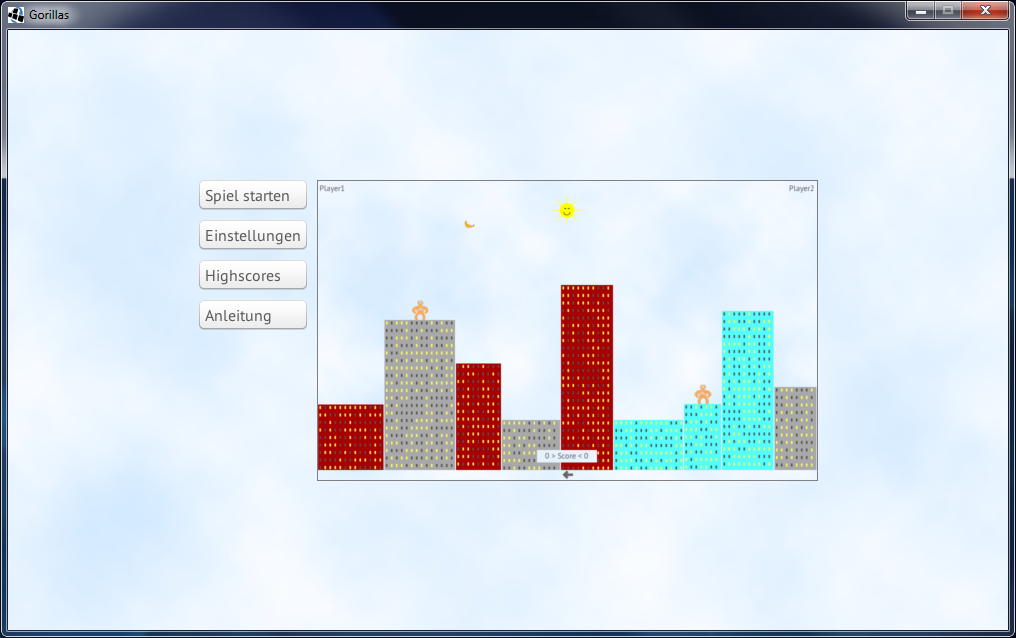
\includegraphics[scale=0.4]{\basepath/\shortGameTitle/menu.png}
\caption{Beispiel einer grafischen Umsetzung des Menüs von \gameTitle}
\label{fig:screenshot1}
\end{center}
\end{figure}

\begin{figure}[htb]
\begin{center}
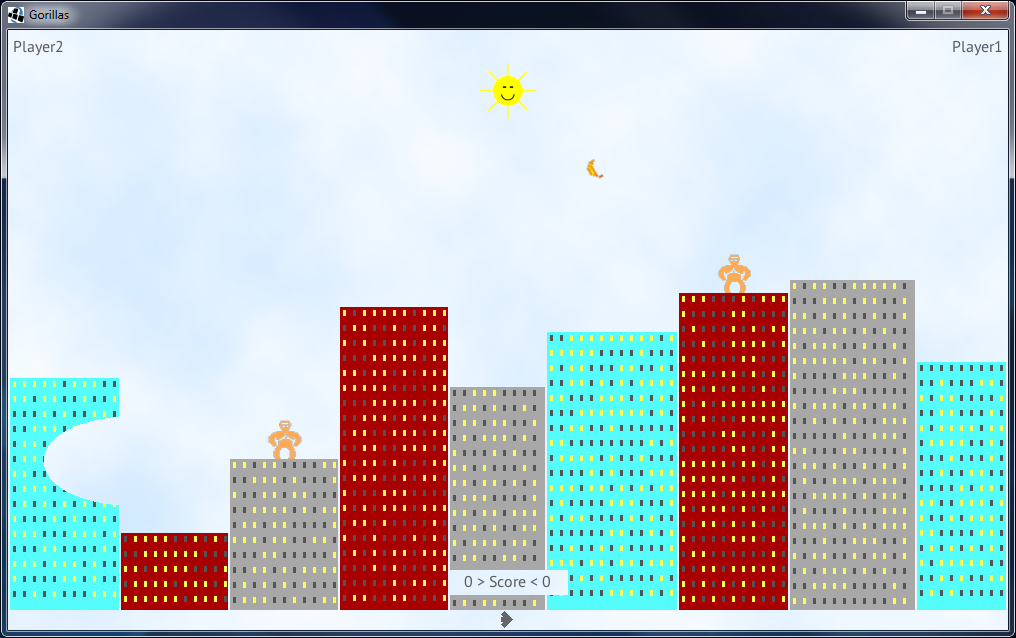
\includegraphics[scale=.4]{\basepath/\shortGameTitle/gameplay.png}
\caption{Beispiel einer grafischen Umsetzung des Spielfensters von \gameTitle}
\label{fig:screenshot2}
\end{center}
\end{figure}

\section{Organisation des Projekts}
\label{sec:orga}

Der offizielle Bearbeitungszeitraum des Projekts beginnt am \emph{\beginDate} und endet am \emph{\finishDate}. 
\myRegister

Die Aufgabenstellung wird etwa \myAvailable, d.h. am \emph{\publishDate}, im Portal ver\"offentlicht. Ab
diesem Zeitpunkt ist prinzipiell bereits die Bearbeitung der Aufgabe m\"oglich. Da zu diesem 
Zeitpunkt die Gruppen im \regSystem noch nicht endg\"ultig gebildet werden konnten, raten wir 
in diesem Fall aber \emph{dringend} zu einer Anmeldung als Gruppe von vier Student\_innen
in der entsprechenden Anmeldung im \regSystem.

Im Projekt bearbeitet die Gruppe die in den folgenden Abschnitten n\"aher definierte Aufgabe. Dabei wird die Gruppe von den Veranstaltern wie folgt unterst\"utzt:

\begin{itemize}

\item Das Portal und insbesondere der neu angelegte Kurs zum \emph{Projekt im \labTerm}\ kann f\"ur alle gruppen\"ubergreifenden Fragen zum Verst\"andnis der Aufgabe oder Unklarheiten bei der Nutzung der Vorlagen genutzt werden.

\item Jede Projektgruppe erh\"alt im Portal eine eigene \emph{Gruppe} sowie ein
\emph{Projektgruppenforum}. In diesem Projektgruppenforum k\"onnen Fragen diskutiert oder
Code-Fragmente ausgetauscht werden (Tipp: umgeben Sie Code im Portal immer mit 
\verb![code java] ...! \verb![/code]!, damit er besser lesbar ist). Da die jeweiligen Tutor\_innen der Gruppe ebenfalls
der Projektgruppe angeh\"oren werden, sind sie in die Diskussionen eingebunden und k\"onnen 
leichter und schneller Feedback geben.

Bitte beachten Sie, dass diese Projektgruppen im Portal von uns nur ein \emph{Angebot} an 
Sie sind, das Sie nicht nutzen m\"ussen. Wenn Sie beispielsweise alle Aufgaben gemeinsam in 
einer WG erledigen, bringt eine Abstimmung \"uber das im 
Portal erstellte Projektgruppenforum vermutlich mehr Aufwand als Nutzen.

\item Eine Gruppe von Tutor\_innen betreut das Projekt. Allen Tutor\_innen wird dabei eine 
gewisse Anzahl Projektgruppen zugeteilt. Die Aufgabe der Tutor\_innen ist es, die Gruppe im Rahmen 
des Projekts bei offenen Fragen zu unterst\"utzen, nicht aber bei der 
tats\"achlichen Implementierung. Insbesondere helfen die Tutor\_innen nicht bei der Fehlersuche 
und geben auch keine L\"osungsvorschl\"age. Die Tutor\_innen stehen der Gruppe auch nur 
zeitlich begrenzt zur Verf\"ugung: pro Gruppe wurden bis zu drei Stunden Betreuung sowie 
eine halbe Stunde f\"ur die Testierung angesetzt.

\item F\"ur den einfacheren Einstieg stellen wir einige Materialien bereit, die
Sie im Portal herunterladen k\"onnen. Diese Materialien inklusive vorgefertigten
Klassen \emph{k\"onnen} Sie nutzen, m\"ussen es aber nicht. Zu den Materialien
z\"ahlen auch vorbereitete Testf\"alle. \emph{Diese \textbf{m\"ussen} unver\"andert auf Ihrer
Implementierung funktionieren, da sie---zusammen mit \glqq{}privaten\grqq{}
Tutorentests---als Basis f\"ur die Abnahme dienen.} Dabei darf auch der Pfad zu
den Testf\"allen \emph{nicht} ver\"andert werden.
\end{itemize}

Wir weisen \emph{ausdr\"ucklich} darauf hin, dass Sie sich \textbf{m\"oglichst fr\"uh} mit den Tests
vertraut machen sollten, um unliebsame \"Uberraschungen \glqq{}kurz vor Fertigstellung\grqq{} zu vermeiden!

Die \emph{Abnahme} oder \emph{Testierung} des Projekts (beschrieben in
Abschnitt \ref{sec:aufgabe}) erfolgt durch den\_die Tutor\_in der Gruppe und erfordert eine
\emph{vorherige Terminabsprache}. Bitte bedenken Sie, dass auch unsere Tutor\_innen
Termine haben (etwa die Abnahme der anderen von ihnen betreuten Gruppen) und
nicht \glqq{}pauschal immer k\"onnen\grqq{}. In Ihrem eigenen Interesse sollten Sie
daher versuchen, so fr\"uh wie m\"oglich einen Termin f\"ur die Besprechungen und 
die Abnahme zu vereinbaren.

Sie sollten auch einen Termin f\"ur die erste Besprechung mit dem\_r Tutor\_in absprechen.
Vor diesem Termin sollten Sie schon dieses Dokument komplett durchgearbeitet haben,
sich alle offenen Fragen notiert haben (und im Portal nach Antworten gesucht haben),
\emph{und} einen Entwurf vorbereitet haben, wie die L\"osung Ihrer Gruppe aussehen soll.
Dieser Entwurf kann in UML erfolgen, aber prinzipiell ist jede (f\"ur den\_die Tutor\_in) lesbare Form
denkbar. Bitte bringen Sie diesen Entwurf zum ersten Treffen mit dem\_der Tutor\_in mit, damit
Sie direkt Feedback erhalten k\"onnen, ob dieser Ansatz funktionieren kann.
Auch hier kann die Nutzung des Portals mit dem Projektgruppenforum helfen, den\_die
Tutor\_in \glqq{}fr\"uher zu erreichen\grqq{}.


\section{Ihre Aufgabe}
\label{sec:aufgabe}

Implementieren Sie eine lauff\"ahige Java-Version des Spiels \emph{\gameTitle}, die
mindestens der \glqq minimalen Ausbaustufe\grqq\ entspricht. 

Das fertige Spiel muss von dem\_der Tutor\_in \emph{vor Ende des Projekts testiert werden}.
Dazu müssen die Dokumentation (etwa 2 DIN A4-Seiten) sowie der Source-Code und
alle zum Übersetzen notwendigen Bibliotheken und Dateien---au\ss{}er den von uns
im Portal bereitgestellten---rechtzeitig vor Ablauf der Einreichung \textbf{von \textit{einem} Gruppenmitglied im Portal hochgeladen werden}.

Das Testat besteht aus den folgenden drei Bestandteilen:

\begin{description}
\item[Live-Test] Der\_die Tutor\_in startet das Spiel und testet, ob alles so funktioniert wie spezifiziert.
Dazu werden potenzielle bestimmte vorgegebene Szenarien durchgespielt, aber auch
zufällig \glqq{}herumgespielt\grqq{}.

\item[Software-Test] Der\_die Tutor\_in testet die Implementierung mit den für alle
Teilnehmer\_innen bereitgestellten (\"offentlichen) und nur f\"ur die Tutor\_innen und
Mitarbeiter\_innen verf\"ugbaren (privaten) JUnit-Tests. Alle Tests m\"ussen
\textbf{ohne Benutzerinteraktion} abgeschlossen werden k\"onnen.

\item[Code-Review] Der\_die Tutor\_in sieht sich den Quellcode sowie die Dokumentation an
und stellt Fragen dazu.
\end{description}


\subsection{Ablauf des Code-Review}
\label{sec:codeReview}

Im Hinblick auf den Code-Review sollten Sie auf gut verst\"andlichen und
dokumentierten Code sowie eine sinnvolle Klassenhierarchie achten, in der Regel
auch mit Aufteilung der Klassen in Packages.

Der\_die Tutor\_in wird einzelne Gruppenmitglieder seiner Wahl zu Teilen des Quelltexts befragen.
Daher sollte sich jedes Gruppenmitglied mit allen Codeteilen auskennen---der\_die Tutor\_in
w\"ahlt aus, zu \emph{welchem Thema} eine Frage gestellt wird und w\"ahlt auch aus, \emph{wer}
die Frage beantworten soll. Die Bewertung dieses Teils bezieht sich also auf die
Aussage eines \glqq{}zuf\"allig ausgew\"ahlten\grqq{} Gruppenmitglieds, geht
aber in die Gesamtpunktzahl der Gruppe ein. 

Damit soll einerseits die \glqq{}Trittbrettfahrerei\grqq{} reduziert werden (\glqq{}ich habe
zwar nichts getan, will aber dennoch die Punkte haben\grqq{}). Gleichzeitig f\"ordert
diese Regelung die Gruppenarbeit, da auch und gerade besonders \glqq{}starke\grqq{}
Mitglieder verst\"arkt R\"ucksicht auf \glqq{}schw\"achere\grqq{} nehmen 
m\"ussen---sonst riskieren sie eine schlechtere Punktzahl, wenn \glqq{}der\_die Falsche\grqq{}
gefragt wird. Durch eine entsprechend bessere Abstimmung in der Gruppe steigen
die Lernm\"oglichkeiten \textbf{aller} Gruppenteilnehmer. Auch für (vermeintliche?)
\glqq{}Expert\_innen\grqq{} wird durch das Nachdenken \"uber die Frage \glqq{}wie erkläre ich das verst\"andlich?\grqq{} das eigene Verst\"andnis vertieft.

\subsection{Dokumentation}
\label{sec:docu}

Neben dem Quelltexten ist auch eine kurze Dokumentation abzugeben (etwa 2 DIN
A4-Seiten). Diese sollte die \emph{Klassenstruktur} ihrer L\"osung in UML umfassen und kurz auf die in ihrer Gruppe \emph{aufgetretenen Probleme} eingehen
sowie \emph{Feedback zur Aufgabenstellung} liefern. Nur die Klassenstruktur geht
in die Bewertung ein; die anderen Elemente helfen uns aber dabei, das Projekt
in der Zukunft besser zu gestalten und sind daher f\"ur uns sehr wichtig. Sie k\"onnen den Teil mit der (hoffentlich konstruktiven) 
Kritik am Projekt auch gerne separat auf Papier---auf Wunsch ohne Angabe des Gruppennamens---dem\_der Tutor\_in geben, wenn Sie das Feedback lieber anonym geben wollen.

Für die Erstellung der Klassendiagramme können Sie beispielsweise die folgenden Tools nutzen:

\begin{itemize}
\item \emph{doxygen} (\url{https://www.doxygen.nl}) ist eine Alternative
zu JavaDoc, die---bei Wahl der entsprechenden Optionen---auch Klassendiagramme
erzeugt. Eine Dokumentation zu \emph{doxygen} finden Sie auf der
obenstehenden Projekt-Homepage.

\item \emph{Fujaba} (\url{https://web.cs.upb.de/archive/fujaba})

\item \emph{BlueJ} (\url{https://bluej.org/})
\end{itemize}

Dies sind nur unsere Empfehlungen. Es steht Ihnen selbstverst\"andlich frei,
andere Tools zu nutzen, etwa OpenOffice Draw oder Microsoft Word. Bitte reichen Sie
die Dokumentation und insbesondere das Klassendiagramm als \textbf{PDF-Datei} ein.

\textbf{Zus\"atzlich} sind mindestens \emph{vier} repr\"asentative Screenshots Ihres Spiels einzureichen, darunter ein Bild vom Startmen\"u.

\subsection{Hinweise}
\label{sec:hinweise}

Denken Sie bitte daran, dass \textbf{Testf\"alle keine Interaktion mit den Spieler\_innen erfordern d\"urfen}.

Sollten Sie sich für die Nutzung des vorgegebenen Frameworks entscheiden, so nutzen Sie das Konzept von Entitäten, Ereignissen und Aktionen. Die Tutor\_innen werden bewerten, wie gut Ihnen das gelungen ist.

Sollten Sie nicht das vorgegebene Framework verwenden, so sollten Sie in Ihrem Code strikt zwischen Logik (Code) und Darstellung (Design) unterscheiden. Die Tutor\_innen werden bewerten, wie gut diese Trennung bei Ihnen gelungen ist.


\subsection{Minimale Ausbaustufe}
\label{sec:minimal}

Um das Projekt bestehen zu k\"onnen, also mindestens 50 aus 100
Punkten zu erhalten, m\"ussen \textbf{alle} nachfolgend genannten Leistungen erbracht werden.

Fehlende Punkte aus der minimalen Ausbaustufe k\"onnen nur in Ausnahmef\"allen ausgeglichen werden.
 % Minimale Ausbaustufe

\begin{description}
\requirement{P\"unktliche Abnahme}{0}{Minimal}{deadline}{\basepath/ontime}

\requirement{Compilierbares Java}{0}{Minimal}{compile} {\basepath/compiles}

\requirement{Nur eigener Code}{0}{Minimal}{ownCode} {\basepath/ownCode}

\requirement{Vorbereitung f\"ur automatisierte Tests}{0}{Minimal}{junit}{\gamepath/junitPrepared}%\gamepath/junitPrepared}

\requirement{\"Offentliche Tests sind erfolgreich}{0}{Minimal}{minimalTest}{\gamepath/public0}

\requirement{Grafische Benutzerschnittstelle}{3}{Minimal}{gui}{\basepath/gui}

\requirement{Hauptmen\"u}{1}{Minimal}{menu}{\gamepath/menu}

\requirement{Neues Spiel starten}{1}{Minimal}{newGame}{\gamepath/newGame}

\requirement{Pause}{1}{Minimal}{pause}{\gamepath/pause}

\requirement{Eingabe und Anzeige der Spielernamen}{6}{Minimal}{playerNames}{\gamepath/playerNames}

\requirement{Grafische Umsetzung der Objekte}{4}{Minimal}{icons}{\gamepath/guiObjects}

\requirement{Platzierung der Gorillas}{3}{Minimal}{gorillaPlacement}{\gamepath/gorillaPlacement}

\requirement{Eingabe der Wurfparameter}{6}{Minimal}{keyboard}{\gamepath/keyboardControl}

\requirement{Wurfverhalten}{8}{Minimal}{shootBehaviour}{\gamepath/shootBehaviour}

\requirement{Erkennen Zugende: Skyline getroffen}{6}{Minimal}{skylineHit}{\gamepath/skylineHit}

\requirement{Erkennen Zugende: Banane verlässt Bildschirm}{4}{Minimal}{leaveScreen}{\gamepath/leaveScreen}

\requirement{Erkennen Zugende: Gegner getroffen}{6}{Minimal}{enemyHit}{\gamepath/enemyHit}


\end{description}


\subsection{Ausbaustufe I}
\label{sec:ausbau1}

Die Ausbaustufe I erweitert die minimale Ausbaustufe. \textbf{Alle
  Anforderungen der minimalen Ausbaustufe gelten weiterhin, sofern sie
  unten nicht explizit ge\"andert oder erweitert werden.}

Bei Implementierung dieser Ausbaustufe k\"onnen insgesamt 75 aus 100
m\"oglichen Punkten erreicht werden. Die \"offentlichen Testf\"alle
f\"ur diese Ausbaustufe befinden sich in der Klasse \texttt{\testLvA}.
 % Ausbaustufe 1

\begin{description} 
\requirement{\"Offentliche Tests der Ausbaustufe 1 sind erfolgreich}{0}{1}{extended1Test}{\gamepath/public1}

\requirement{Sinnvolle Modellierung}{5}{1}{\basepath/mvc}{\basepath/mvc}

\requirement{Highscore-Liste}{5}{1}{highscoreDB}{\gamepath/highscore}

\requirement{Highscore GUI}{5}{1}{highscoreGUI}{\gamepath/highscoreGUI}

\requirement{Rundenbasiertes Spiel: Kartengenerator}{5}{1}{mapgenerator}{\gamepath/mapgenerator}

\requirement{Rundenbasiertes Spiel: Spiel bis 3 und Score-Anzeige}{3}{1}{score}{\gamepath/score}

\requirement{Wurfparameter werden gespeichert}{2}{1}{parametersaved}{\gamepath/parametersaved}

\end{description}


\subsection{Ausbaustufe II}

Die Ausbaustufe II erweitert Ausbaustufe I und die minimale
Ausbaustufe. \textbf{Alle Anforderungen dieser Ausbaustufen gelten
  weiterhin, sofern sie unten nicht explizit ge\"andert oder erweitert
  werden.}

Bei Implementierung dieser Ausbaustufe k\"onnen insgesamt 90 aus 100
m\"oglichen Punkten erreicht werden. Die \"offentlichen Testf\"alle
f\"ur diese Ausbaustufe befinden sich in der Klasse \texttt{\testLvB}.
 % Ausbaustufe 2

\begin{description}
\requirement{\"Offentliche Tests der Ausbaustufe 2 sind erfolgreich}{0}{2}{extended2Test}{\gamepath/public2}

\requirement{Wind}{5}{2}{wind}{\gamepath/wind}

\requirement{Dotzen}{5}{2}{bounce}{\gamepath/bounce}

\requirement{Sonne}{3}{2}{sun}{\gamepath/sun}

\requirement{Spieler\_innennamen werden gespeichert}{2}{2}{namessaved}{\gamepath/namessaved}


\end{description}


\subsection{Ausbaustufe III}

Die Ausbaustufe III erweitert Ausbaustufe II, I und die minimale
Ausbaustufe. \textbf{Alle Anforderungen dieser Ausbaustufen gelten
  weiterhin, sofern sie unten nicht explizit ge\"andert oder erweitert
  werden.}

Bei Implementierung dieser Ausbaustufe k\"onnen insgesamt 100 aus 100
m\"oglichen Punkten erreicht werden. Die \"offentlichen Testf\"alle
f\"ur diese Ausbaustufe befinden sich in der Klasse \texttt{\testLvC}.
 % Ausbaustufe 3

\begin{description}

\requirement{\"Offentliche Tests der Ausbaustufe 3 sind erfolgreich}{0}{3}{extended3Test}{\gamepath/public3}

\requirement{Erdbeschleunigung kann verändert werden}{4}{3}{gravity}{\gamepath/gravity}

\requirement{Spöttische Bemerkungen}{4}{3}{incitingmessages}{\gamepath/incitingmessages}

\requirement{Anleitung}{2}{3}{instructions}{\gamepath/instructions}

\end{description}

\subsection{Anpassungen f\"ur Studierende im Studiengang CE}

Die Anforderungen f\"ur Studierende im Studiengang CE ersetzen Teile der Ausbaustufe I-III, wie unten erl\"autert. Dabei sind zwei Aspekte
umzusetzen: eine \emph{realistische Flugbahn unter Ber\"ucksichtigung der Luftreibung} sowie \emph{(semi-)dynamische Windb\"oen}.

\emph{Achtung:} die Anforderung \glqq{}Wurfverhalten\grqq{} der minimalen Ausbaustufe ist zus\"atzlich \emph{unver\"andert} zu
implementieren, da sonst zahlreiche Tests scheitern. Gehen Sie dazu so vor, dass in Ihrem Spiel \emph{zwei} Funktionen zur
Berechnung der Flugbahn existieren. Das \emph{Spiel} selbst soll die realistischere, aber komplexere Formel nutzen, w\"ahrend die
\emph{Tests} auf das vereinfachte \glqq{}Wurfverhalten\grqq{} zur\"uckgreifen.

Die folgenden Anforderungen gelten f\"ur Studierende im Studiengang Computational Engineering (CE) sowie f\"ur gemischte Gruppen, an denen
CE-Studierende beteiligt sind. Dabei geh\"oren die ersten beiden Punkte zusammen:

\begin{description}
\item[Die parabolische Flugbahn] soll die Luftreibung wie folgt ber\"ucksichtigen:

\begin{equation*}
F = 0.5 \cdot \rho \cdot C \cdot A \cdot V^2
\end{equation*}

mit 

\begin{itemize}
\item A = Fläche der Banane 
\item $\rho$ = Dichte (1.293 $\frac{kg}{m^2}$) bei 0° Celsius und 1 Atmosphere Luftdruck) 
\item C = 2.1 
\item V = Geschwindigkeit relativ zur Luftgeschwindigkeit, d.h. $v(t) - v_{luft}(t)$.
\end{itemize}

Auf die Ber\"ucksichtigung der Rotation der Banane kann verzichtet werden.

\item[Die Berechnung des Bananenflugs] soll entweder das Runge-Kutte-Verfahren\footnote{siehe \url{http://de.wikipedia.org/wiki/Runge-Kutta-Verfahren}}
oder symplektische Euler-Integration wie folgt verwendet werden: 

\begin{eqnarray*}
a(t) & = & F(v(t), x(t), t)\\
v(t+1) &=& v(t) + dt \cdot a(t)\\
x(t+1) &=& x(t) + dt \cdot v(t+1)
\end{eqnarray*}


\item[Windb\"oen] wehen mit einer eigenen Luftgeschwindigkeit 
 $v_{luft}(t) = v_l \cdot sin(2 \cdot \pi \cdot t / D)$, wobei $v_l$ und $D$ Zufallszahlen sind. Bestimmen Sie f\"ur die Zufallszahlen durch Ausprobieren
 und/oder entsprechende \"Uberlegungen eine passende Begrenzung, um unrealistisch starke Winde oder unglaubw\"urdige Windrichtungen m\"oglichst
 auszuschlie\ss{}en. 

\textbf{Hinweis}: Die Windb\"oben sollen innerhalb eines Spielzugs---also von dem Zeitpunkt des Spielerwechsels bis zum Ende der Flugbahn der geworfenen
Banane---\emph{konstant} bleiben, wechseln also erst mit dem n\"achsten Spielzug. Dies ist zwar nur bedingt realistisch, erm\"oglicht aber die \glqq{}Spielbarkeit\grqq{}.
Bei (realistischen) dynamischen Windb\"oen, die auch w\"ahrend der Eingabe der Flugparameter und w\"ahrend des Flugs ihre St\"arke und/oder Richtung
variieren k\"onnen, k\"onnen an sich pr\"azise ausgerechnete W\"urfe das Ziel verfehlen---und gleichzeitig ziemlich falsch berechnete Werte \glqq{}zuf\"allig
treffen\grqq{}. Damit w\"are Gorillas effektiv unspielbar, da der Zufall eine zu gro\ss{}e Rolle spielen w\"wurde.
\end{description}

Die beiden ersten Aspekte (\glqq{}Parabolische Flugbahn mit Luftreibung und realistischer Berechnung\grqq{} ersetzen insgesamt die
beiden Anforderungen \glqq{}Erdbeschleunigung kann ver\"andert werden\grqq{} und \glqq{}Sp\"ottische Bemerkungen\grqq{} aus Aufbaustufe III und ergeben
daher 8 Punkte. 

Die Anforderung \glqq{}Windb\"oen\grqq{} ersetzt f\"ur CE-Gruppen die Anforderung \glqq{}Sonne\grqq{} und ergibt damit 3 Punkte.

\glqq{}Nicht-CE-Gruppen\grqq{}, die diese Aufgaben (korrekt) bearbeiten, erhalten die genannten Punktzahlen als \emph{Bonuspunkte}. Analog
erhalten CE-Gruppen, die die \glqq{}gestrichenen\grqq{} Aufgabenteile (korrekt) bearbeiten, die entsprechende Punktzahl als Bonuspunkte.

Bitte beachten Sie, dass die obigen Aufgaben \emph{nicht} Bestandteil der Testf\"alle sind. Weicht das von Ihnen berechnete Verhalten von der (einfacheren)
allgemeinen Formel ab, werden die entsprechenden Tests entsprechend fehlschlagen. Dadurch m\"ussen Sie nicht in Panik geraten; ihr\_e Tutor\_in wird Ihre
Implementierung dieser Aspekte im Code begutachten und bewerten. Denken Sie an den Tip mit den \glqq{}zwei Varianten\grqq{}, um Fehler in den Tests zu vermeiden!


\subsection{Optionale Aufgabe im Bereich Wirtschaft}

Unterstellen Sie f\"ur diese Aufgabe, dass Ihr Spiel die Aufgabenstellung
vollst\"andig und \glqq{}mit sch\"oner Optik\grqq{} (h\"ubsche Bilder, gute Soundeffekte etc.) umsetzt.
	
Legen Sie sich nun auf einen (theoretischen) Vermarktungsweg f\"ur ihr Spiel fest. Zur Wahl stehen insbesondere
der \emph{iTunes Store} (iOS-Anwendungen), der \emph{Google Play Store} (Android), der \emph{Mac App Store} (Mac-Anwendungen),
sowie der Microsoft Store (Windows 10-Anwendungen)---im Folgenden kurz als \glqq{}Store\grqq{} abstrahiert\footnote{Ignorieren
	Sie f\"ur die Bearbeitung dieser Aufgabe, dass das von Ihnen geschriebene Spiel in der vorliegenden Fassung in der
	Regel so in keinen der genannten Stores eingestellt werden kann (nicht direkt lauff\"ahig unter iOS oder Android, ...)}.
	
Finden Sie f\"ur den von Ihnen gew\"ahlten \emph{Store} heraus, welche Vermarktungsm\"oglichkeiten und
welche Preisstaffelungen es gibt. So stehen z.B. im \emph{iTunes Store} nur bestimmte Preise zur Verf\"ugung.
Recherchieren Sie zudem, welche Angebotsm\"oglichkeiten es gibt (Vollversion, Demoversion mit Kaufangebot, In-App-K\"aufe,
integrierte Werbung, ...). Bestimmen Sie ebenfalls, welchen Anteil an den Kaufpreisen (mit Ausnahme von Gratisangeboten)
der Store-Betreiber einbeh\"alt.
	
Suchen Sie in dem gew\"ahlten Store nach verwandten oder vergleichbaren Spielen und betrachten Sie deren Preisgestaltung.

Entscheiden Sie sich anhand der so zusammengetragenen Informationen nun f\"ur eine Ihnen geeignet erscheinende Vermarktung. Ihr
Ziel sollte (nat\"urlich) die Erzielung des maximal m\"oglichen Gewinns sein.

Bestimmen Sie angesichts der von Ihnen recherchierten Preis- und Bereitstellungsmodelle, des Betreiberanteils und der
\glqq{}Konkurrenzangebote\grqq{} das aus Ihrer Sicht beste Vermarktungsmodell. Fassen Sie die gewonnenen Erkenntnisse zu den 
genannten Punkten in einer kurzen Dokumentation zusammen, die mindestens die folgenden Angaben enth\"alt:
	
\begin{itemize}
\item Gew\"ahlter Store
\item Recherchierte verf\"ugbare Vermarktungsoptionen (Vollversion, Demo mit Upgrade, ...)
\item Recherchierte verf\"ugbare Preisstaffelungen
\item Anteil der Einnahmen, die an den Betreiber flie\ss{}en
\item Recherchierte Konkurrenzprodukte mit Preisgestaltung (mindestens drei)
\item Begr\"undete (!) Festlegung auf die Ihnen am besten erscheinende Vermarktung.		
\end{itemize}

Bitte versuchen Sie, die Dokumentation verst\"andlich und nachvollziehbar, aber auch so knapp wie m\"oglich zu halten. Es soll
kein Roman werden---in der Regel sollten 2-4 Seiten ausreichen! Zu dieser Aufgabe gibt es keine
\glqq{}Musterl\"osung\grqq{}---Ihre Punktzahl (max. 10 Punkte) bestimmt sich daran, wie vollst\"andig und \"uberzeugend
Ihre Recherche und die Begr\"undung der letzlichen Entscheidung ist.
	
Bitte beachten Sie, dass diese Bearbeitung \emph{ausschlie\ss{}lich theoretisch (\glqq{}auf Papier\grqq{})} erfolgt. Es wird also
weder \glqq{}Code geschrieben\grqq{} noch sollen Sie wirklich versuchen, das Spiel \glqq{}online zu stellen\grqq{}! 


\subsection{Bonuspunkte}

Sie k\"onnen auch mehr als 100 Punkte erreichen sowie fehlende Punkte
aus anderen Ausbaustufen ausgleichen, indem Sie weitere Funktionen
implementieren, die in den Ausbaustufen nicht spezifiziert wurden. Die
Bewertung ist dabei Sache der Tutor\_innen und der Veranstalter\_innen. Zur
Orientierung stellen wir hier beispielhaft m\"ogliche Erweiterungen mit
Punktzahl vor, damit Sie wissen, was wir ungef\"ahr erwarten.
 % Bonuspunkte

\begin{description}
\requirement{Nutzung von Audio-Clips}{1}{Bonus}{audio}{\basepath/audio}

\requirement{\glqq{}About\grqq-Fenster}{1}{Bonus}{aboutBox}{\basepath/about}

\requirement{\"Uberraschen Sie uns}{0}{Bonus}{surprise}{\basepath/surprise}

\end{description}

\textbf{Hinweis:} Der Code in den Testklassen \textbf{darf auf keinen Fall} zur Anzeige von
Dialogfenstern f\"uhren. Dies darf auch bei inkorrekten Schritten nicht geschehen, da sonst eine Eingabe erfordert w\"urde, die in den JUnit-Tests nicht automatisiert erfolgen kann. Zum Testen darf nicht der \textit{org.newdawn.slick.AppGameContainer} werden, da dieser zur Anzeige von Dialogfenstern führt. Verwenden Sie stattdessen \textit{de.tu\_darmstadt.gdi1.gorillas.tests.TestAppGameContainer}.

Die Tests benutzen weiterhin nicht die Klasse \textit{de.tu\_darmstadt.informatik.fop.gorillas.main.Gorillas} sondern die Klasse \textit{
de.tu\_darmstadt.gdi1.gorillas.test.setup.TestGorillas}. Diese Klasse erbt statt von \textit{org.slick.StateBasedGame} von \textit{de.tu\_darmstadt.informatik.fop.gorillas.test.setup.TWLTest\allowbreak StateBasedGame}. Sie müssen folglich exakt wie Sie in der Klasse Gorillas Ihre States hinzugefügt haben, dies auch in TestGorillas tun. TWLTestStateBasedGame verzichtet im Gegensatz zu TWLStateBasedGame auf das Rendern der TWL-GUI-Elemente.

Bitte achten Sie bei den Erweiterungen darauf, dass alte Funktionalität nicht verloren geht.


\section{Materialien}

Auf der Veranstaltungsseite stellen wir Ihnen einige Dateien zur Verf\"ugung, die Sie f\"ur Ihre L\"osung verwenden k\"onnen. Dabei handelt es sich um vorgefertigte Karten und
die \"offentlichen Testf\"alle. Es wird Ihnen dringend nahe gelegt, auch unser bereitgestelltes Framework nutzen. Das Framework ist threadsicher!

\textbf{Hinweis:} Sie dürfen auch eine vollst\"andig eigene L\"osungen implementieren. Der dadurch entstehende Mehraufwand wird aber nicht durch Punkte gewürdigt. Ihre L\"osung \textbf{muss} in jedem Fall mit den bereitgestellten Testklassen \"uberpr\"ufbar sein.

Neben der kurzen Beschreibung in diesem Dokument gibt Ihnen die
JavaDoc-Dokumentation n\"utzliche Hinweise zur Verwendung und den
Parametern der vorhandenen Funktionen. Ein Blick in diese Quellen empfiehlt sich
sehr---\textbf{am besten vor dem Gang zum\_zur Tutor\_in}, um$\ldots$

\begin{itemize}
\item sich selbst und auch dem\_der Tutor\_in wertvolle Zeit zu sparen, da sich so unter Umst\"anden banale Fragen von selbst l\"osen,

\item Nerven zu sparen, da das Warten auf die Antwort der Tutor\_innen Ihre Nerven beanspruchen wird :-),

\item sich selbstst\"andiges Arbeiten anzueignen.
\end{itemize} 


\subsection{Klasse \emph{de.tu\_darmstadt.informatik.fop.gorillas.main.Gorillas}}

\textit{\gameTitle} erbt von \textit{org.slick.StateBasedGame}. \textit{\gameTitle} dient sowohl als Container für Spiele 
als auch zum Starten des gesamten Spiels. Sie müssen diese Klasse erweitern, um zusätzliche States hinzuzufügen. Lesen Sie sich dazu das \tutorialURL durch.

\subsection {Die ersten Schritte}
Sie sollten sich zunächst das  \tutorialURL 
durchlesen, um das Konzept des Frameworks zu verstehen. Anschließend können Sie in \texttt{\gameTitle} zusätzliche 
States (Fenster) definieren. Sie sollten mit einem Hauptmenü und einem Spielfenster beginnen.

Anschließend sollten Sie in der Gruppe diskutieren, wie Ihr Projekt strukturiert werden soll und Aufgaben in der Gruppe verteilen.

% basicevents
\subsection {Basisereignisse und Basisaktionen}

Das \textbf{eea}-Framework arbeitet mit \textbf{Entit\"aten}, wie der \textbf{ImageRenderComponent}, sowie \textbf{Events} und
zugehörigen \textbf{Actions}. Die zwei Tabellen am Ende geben einen Überblick über die mitgelieferten Events und Actions.
Das Neuzeichnen eines Fensters geschieht zusammen mit einem Frame.

\begin{table}[htbp]
\begin{tabular}{|p{.45\textwidth}|p{.5\textwidth}|}\hline

\textbf{Konstruktor} & \textbf{Beschreibung}\\\hline\hline
\emph{CollisionEvent()} & Dieses Event wird (mit jedem Frame) ausgelöst, wenn sich zwei Entitäten überlappen.\\\hline
\emph{KeyPressedEvent(String id, Integer... key)} & Dieses Event wird ausgelöst, wenn die Taste gerade erstmalig nach unten gedrückt wurde.\\\hline
\emph{KeyDownEvent(String id, Integer... key)} & Dieses Event wird ausgelöst, wenn die Taste aktuell unten gehalten wird.\\\hline
\emph{LeavingScreenEvent()} & Dieses Event wird ausgelöst, wenn die an diesem Event interessierte Entität die Spielfl\"ache verlassen hat.\\\hline
\emph{LoopEvent(String id)} & Dieses Event wird mit jedem Frame ausgelöst. Dieses Event eignet sich also dafür, in jedem Frame eine gewisse Aktion auszuführen.\\\hline
\emph{MouseClickedEvent()} & Dieses Event wird ausgelöst, wenn die Maus auf die an dem Event interessierte Entität geklickt hat.\\\hline
\emph{MouseEnteredEvent()} & Dieses Event wird ausgelöst, wenn die Maus über die an dem Event interessierte Entität fährt.\\\hline
\emph{MovementDoesntCollideEvent(float speed, IMovement move)} & Dieses Event wird ausgelöst, wenn die Bewegung (Action) keine Kollision mit einer anderen Entität verursacht.\\\hline

\end{tabular}
\caption{Basisereignisse des \textbf{eea}-Frameworks aus dem package \emph{eea.engine.events.basicevents}}
\end{table}

% basicevents
%\subsection {Basisaktionen}

\begin{table}[htbp]
\begin{tabular}{|p{.4\textwidth}|p{.5\textwidth}|}\hline
\textbf{Konstruktor} & \textbf{Beschreibung}\\\hline\hline
\emph{ChangeStateAction(int state)} & Diese Action wechselt in einen Zustand (State) mit der State-ID \textbf{state}. Ist der State schon einmal initialisiert worden, so wird die \textbf{init}-Methode nicht erneut aufgerufen.\\\hline
\emph{ChangeStateInitAction(int state)} & Diese Action wechselt in einen State mit der State-ID state. Auch wenn der State schon einmal initialisiert worden ist, 
wird die \textbf{init}-Methode erneut aufgerufen.\\\hline
\emph{DestroyEntityAction()} & Diese Action zerstört die Entität bei Eintreten eines gewissen Events.\\\hline
\emph{MoveBackwardAction(float speed)*} & Diese Action führt mit einer Geschwindigkeit \textbf{speed} eine Rückwärtsbewegung entgegen der Blickrichtung aus.\\\hline
\emph{MoveDownAction(float speed()*} & Diese Action führt mit einer Geschwindigkeit \textbf{speed} eine Bewegung nach unten aus.\\\hline
\emph{MoveForwardAction(float speed)*} & Diese Action führt mit einer Geschwindigkeit \textbf{speed} eine Vorwärtsbewegung in Blickrichtung aus.\\\hline
\emph{MoveLeftAction(float speed)*} & Diese Action führt mit einer Geschwindigkeit \textbf{speed} eine Bewegung nach links aus.\\\hline
\emph{MoveRightAction(float speed)*} & Diese Action führt mit einer Geschwindigkeit \textbf{speed} eine Bewegung nach rechts aus.\\\hline
\emph{MoveUpAction(float speed)*} & Diese Action führt mit einer Geschwindigkeit \textbf{speed} eine Bewegung nach oben aus.\\\hline
\emph{RotateLeftAction(float speed)*} & Diese Action führt mit einer Geschwindigkeit \textbf{speed} eine Drehung nach links aus.\\\hline
\emph{RotateRightAction(float speed)*} & Diese Action führt mit einer Geschwindigkeit \textbf{speed} eine Drehung nach rechts aus.\\\hline
\emph{QuitAction()} & Diese Action beendet das laufende Spiel.\\\hline
\emph{RemoveEventAction()} & Diese Action zerstört ein Event.\\\hline
\emph{SetEntityPositionAction(Vector2f pos)} & Diese Action setzt die Position einer Entität neu.\\\hline

\end{tabular}
\caption{Basisaktionen des \textbf{eea}-Frameworks aus dem package \emph{eea.engine.actions.basicactions.} Die mit einem * markierten Aktionen sind für das Spiel \gameTitle nicht von Bedeutung. Um den Wurf eines Objektes zu simulieren, empfiehlt es sich eine eigene MoveAction zu implementieren. Die Richtungen werden verdeutlicht durch Abbildung \vref{fig:screenshot3}.}
\end{table}

\begin{figure}[htbp]
\begin{center}

\includegraphics[width=7cm]{\basepath/\shortGameTitle/directions.png}
\caption{Es gibt zahlreiche Aktionen, die eine Bewegung ausdrücken.}
\label{fig:screenshot3}
\end{center}
\end{figure}


\section{Zeitplanung}
\label{sec:zeitplanung}

Wir empfehlen Ihnen, \textbf {vor Beginn der Bearbeitung} zuerst eine f\"ur Ihre
Gruppe realistische Ausbaustufe auszuw\"ahlen und die Aufgabe dann in parallel
bearbeitbare Teilaufgaben zu zerlegen, die Sie auf die einzelnen Gruppenmitglieder
verteilen. \"Uber zentrale Elemente wie die grunds\"atzlichen Klassennamen und die
Vererbungshierarchie sollten Sie sich in der Gruppe einigen, um sp\"atere Diskussionen zu vermeiden.

Erstellen Sie einen schriftlichen Zeitplan, wann Sie welche Aufgabe abgeschlossen
haben m\"ochten. Dabei ist es wichtig, den aktuellen Projektstand regelm\"a\ss{}ig
kritisch zu \"uberpr\"ufen. Ein solches geplantes Vorgehen vermeidet Stress (und damit unn\"otige Fehler) beim Abgabetermin.

Eine Zeitplanung f\"ur die minimale Ausbaustufe k\"onnte etwa wie in Tabelle
\vref{tab:zeitplanMinimal} gezeigt aussehen. Eine denkbare Gesamteinteilung f\"ur
alle Ausbaustufen wird in Tabelle \vref{tab:zeitplanAlles} gezeigt.

Bitte beachten Sie, dass \textbf{alle Zeiten stark von Ihrem Vorwissen und Ihren
F\"ahigkeiten abh\"angen}, so dass die Zeiten nicht als \glqq{}verbindlich\grqq{} betrachtet werden d\"urfen!

\begin{table}[htb]
\begin{center}\begin{tabular}{|p{.75\textwidth}|r|}\hline
\textbf{Aspekt} & \textbf{Aufwand (ca.)}\\\hline\hline

Einarbeitung in die Aufgabenstellung und Vorlagen, Lesen des Tutorials & 1.5 Tage\\\hline

Einigung auf die grunds\"atzliche Klassen- und Packagehierarchie & 0.25 Tage\\\hline

Entwicklung der grafischen Benutzerschnittstelle (Spielfenster und Menüfenster) & 0.25 Tag\\\hline

Neues Spiel per Tastendruck & 0.1 Tag\\\hline

Eingabe und Anzeige der Spielernamen & 0.5 Tag\\\hline

Umsetzung der grafischen Objekte & 0.1 Tag\\\hline

Eingabe der Wurfparameter & 0.3 Tag\\\hline

Wurfverhalten & 0.5 Tag \\\hline

Erkennen Zugende: Skyline getroffen & 0.25 Tag \\\hline

Erkennen Zugende: Banane verl\"asst Bildschirm & 0.1 Tag \\\hline

Erkennen Zugende: Gegner getroffen & 0.25 Tag \\\hline
\end{tabular}
\caption{Zeitplanung f\"ur die Bearbeitung \glqq{}nur\grqq{} der minimalen Ausbaustufe.
Die Aufgaben werden in der Regel parallel von einzelnen oder mehreren Gruppenmitgliedern bearbeitet.}
\label{tab:zeitplanMinimal}
\end{center}
\end{table}

\begin{table}[htb]
\begin{center}
\begin{tabular}{|p{.25\textwidth}|p{.65\textwidth}|}\hline
\textbf{Stufe} & \textbf{Gesch\"atzter Zeitumfang}\\\hline\hline
   Minimale Ausbaustufe & 4 - 5 Tage \\\hline

   Ausbaustufe I & 3 - 4 Tage \\\hline

   Ausbaustufe II & 2 - 3 Tage \\\hline

   Ausbaustufe III & 1 - 2 Tage \\\hline

   Bonusaufgaben & Falls hier von Anfang an ein \emph{starkes} Interesse bestehen
   sollte, sollten Sie sich am besten vom ersten Tag an Gedanken machen und m\"oglichst z\"ugig anfangen...\\\hline
\end{tabular}
\caption{Zeitplanung f\"ur die Bearbeitung aller Ausbaustufen mit 4 Personen}
\label{tab:zeitplanAlles}
\end{center}
\end{table}

\textbf{Tipp}: Wenn Sie eine Ausbaustufe fertig implementiert haben, sollten Sie
einen Gang zum\_zur Tutor\_in nicht scheuen, ehe Sie sich gleich an die n\"achste Stufe
heranwagen. Fragen Sie Ihre\_n Tutor\_in nach eventuellen Unklarheiten, falls Sie z. B.
inhaltlich die Aufgabenstellung nicht verstanden haben. Es ist Aufgabe der Tutor\_innen,
Fragen zu beantworten, also nutzen Sie dieses Angebot.

\textbf{Wichtig:} \glqq{}Sichern\grqq{} Sie stabile Zwischenergebnisse, etwa indem
Sie ein Versionskontrollverfahren wie \emph{SVN} oder \emph{Git} nutzen. Tipps dazu
finden Sie im Portal. Die einfache Variante ist es, regelm\"a\ss{}ig eine JAR-Datei
mit den Quellen (!) anzulegen, die Sie jeweils je nach erreichtem Status \glqq{}passend\grqq{}
benennen. Dann haben Sie immer eine R\"uckfallm\"oglichkeit, falls etwa nach einem Code-Umbau nichts mehr funktioniert.


%\subsection{Anpassungen f\"ur Studierende im Studiengang CE}

Die Anforderungen f\"ur Studierende im Studiengang CE ersetzen Teile der Ausbaustufe I-III, wie unten erl\"autert. Dabei sind zwei Aspekte
umzusetzen: eine \emph{realistische Flugbahn unter Ber\"ucksichtigung der Luftreibung} sowie \emph{(semi-)dynamische Windb\"oen}.

\emph{Achtung:} die Anforderung \glqq{}Wurfverhalten\grqq{} der minimalen Ausbaustufe ist zus\"atzlich \emph{unver\"andert} zu
implementieren, da sonst zahlreiche Tests scheitern. Gehen Sie dazu so vor, dass in Ihrem Spiel \emph{zwei} Funktionen zur
Berechnung der Flugbahn existieren. Das \emph{Spiel} selbst soll die realistischere, aber komplexere Formel nutzen, w\"ahrend die
\emph{Tests} auf das vereinfachte \glqq{}Wurfverhalten\grqq{} zur\"uckgreifen.

Die folgenden Anforderungen gelten f\"ur Studierende im Studiengang Computational Engineering (CE) sowie f\"ur gemischte Gruppen, an denen
CE-Studierende beteiligt sind. Dabei geh\"oren die ersten beiden Punkte zusammen:

\begin{description}
\item[Die parabolische Flugbahn] soll die Luftreibung wie folgt ber\"ucksichtigen:

\begin{equation*}
F = 0.5 \cdot \rho \cdot C \cdot A \cdot V^2
\end{equation*}

mit 

\begin{itemize}
\item A = Fläche der Banane 
\item $\rho$ = Dichte (1.293 $\frac{kg}{m^2}$) bei 0° Celsius und 1 Atmosphere Luftdruck) 
\item C = 2.1 
\item V = Geschwindigkeit relativ zur Luftgeschwindigkeit, d.h. $v(t) - v_{luft}(t)$.
\end{itemize}

Auf die Ber\"ucksichtigung der Rotation der Banane kann verzichtet werden.

\item[Die Berechnung des Bananenflugs] soll entweder das Runge-Kutte-Verfahren\footnote{siehe \url{http://de.wikipedia.org/wiki/Runge-Kutta-Verfahren}}
oder symplektische Euler-Integration wie folgt verwendet werden: 

\begin{eqnarray*}
a(t) & = & F(v(t), x(t), t)\\
v(t+1) &=& v(t) + dt \cdot a(t)\\
x(t+1) &=& x(t) + dt \cdot v(t+1)
\end{eqnarray*}


\item[Windb\"oen] wehen mit einer eigenen Luftgeschwindigkeit 
 $v_{luft}(t) = v_l \cdot sin(2 \cdot \pi \cdot t / D)$, wobei $v_l$ und $D$ Zufallszahlen sind. Bestimmen Sie f\"ur die Zufallszahlen durch Ausprobieren
 und/oder entsprechende \"Uberlegungen eine passende Begrenzung, um unrealistisch starke Winde oder unglaubw\"urdige Windrichtungen m\"oglichst
 auszuschlie\ss{}en. 

\textbf{Hinweis}: Die Windb\"oben sollen innerhalb eines Spielzugs---also von dem Zeitpunkt des Spielerwechsels bis zum Ende der Flugbahn der geworfenen
Banane---\emph{konstant} bleiben, wechseln also erst mit dem n\"achsten Spielzug. Dies ist zwar nur bedingt realistisch, erm\"oglicht aber die \glqq{}Spielbarkeit\grqq{}.
Bei (realistischen) dynamischen Windb\"oen, die auch w\"ahrend der Eingabe der Flugparameter und w\"ahrend des Flugs ihre St\"arke und/oder Richtung
variieren k\"onnen, k\"onnen an sich pr\"azise ausgerechnete W\"urfe das Ziel verfehlen---und gleichzeitig ziemlich falsch berechnete Werte \glqq{}zuf\"allig
treffen\grqq{}. Damit w\"are Gorillas effektiv unspielbar, da der Zufall eine zu gro\ss{}e Rolle spielen w\"wurde.
\end{description}

Die beiden ersten Aspekte (\glqq{}Parabolische Flugbahn mit Luftreibung und realistischer Berechnung\grqq{} ersetzen insgesamt die
beiden Anforderungen \glqq{}Erdbeschleunigung kann ver\"andert werden\grqq{} und \glqq{}Sp\"ottische Bemerkungen\grqq{} aus Aufbaustufe III und ergeben
daher 8 Punkte. 

Die Anforderung \glqq{}Windb\"oen\grqq{} ersetzt f\"ur CE-Gruppen die Anforderung \glqq{}Sonne\grqq{} und ergibt damit 3 Punkte.

\glqq{}Nicht-CE-Gruppen\grqq{}, die diese Aufgaben (korrekt) bearbeiten, erhalten die genannten Punktzahlen als \emph{Bonuspunkte}. Analog
erhalten CE-Gruppen, die die \glqq{}gestrichenen\grqq{} Aufgabenteile (korrekt) bearbeiten, die entsprechende Punktzahl als Bonuspunkte.

Bitte beachten Sie, dass die obigen Aufgaben \emph{nicht} Bestandteil der Testf\"alle sind. Weicht das von Ihnen berechnete Verhalten von der (einfacheren)
allgemeinen Formel ab, werden die entsprechenden Tests entsprechend fehlschlagen. Dadurch m\"ussen Sie nicht in Panik geraten; ihr\_e Tutor\_in wird Ihre
Implementierung dieser Aspekte im Code begutachten und bewerten. Denken Sie an den Tip mit den \glqq{}zwei Varianten\grqq{}, um Fehler in den Tests zu vermeiden!


\section{Liste der Anforderungen}
\listofrequirements

\end{document}
